%!TeX root=./tese.tex
% A2 MERGE: absorbs the former aiconfigurator.tex, twopool.tex and
% validation.tex (deleted at finalize). Figures: figuras/aic/ (from
% collector_artifacts/phaseA-C) and figuras/sim/ (simulation/sweep_fig.py,
% simulation/burst_queue_fig.py). Live-anchor artifacts:
% simulation/results/live51/; harness simulation/live51/. Numbers from the
% provenance DB (current_* views) and progress/results-ledger.md. Detail
% displaced by the merge lives in the supplementary archive (S3/S4),
% indexed from Appendix ap:artifacts.
\chapter{Methodology and Platform}
\label{cap:metodologia}%
% Aliases: the merged chapters' identifiers travel with their content and
% keep resolving to this chapter (aiconfigurator / twopool / validation).
\label{cap:aiconfigurator}%
\label{cap:twopool}%
\label{cap:validation}%
\chaptermark{Methodology and Platform}

The platform every later result runs on has three layers, each calibrated and
then checked
against something outside itself: an analytical cost model for the vision
stage, collected on this thesis's own silicon and validated against physical
measurement of the real network (Section~\ref{sec:aic-collection}); a
two-pool discrete-event composition running the production trace end to end,
with the language pool priced by NVIDIA's shipped H100 database
(Section~\ref{sec:aic-twopool}); and a live-stack anchor replaying two of
the thesis's own policies through Dynamo's real control plane
(Section~\ref{sec:val-results}). None of these is a research question; they
are the ground the research questions stand on. What the platform reproduces
faithfully and what it does not is stated once, in
Section~\ref{sec:sim-limitations}.

\section{The replay platform: trace, converter, and the two-pool seam}
\label{sec:sim-arch}

Every experiment is driven by the same substrate, Microsoft's
\textit{AzureLMMInferenceDataset2025}~\cite{AzureLMM2025}, characterized in
Chapter~\ref{cap:trace-eda}: seven days, one million requests, four fields
per request (arrival timestamp, image count, context tokens, generated
tokens). No request bodies exist, so all simulated work is reconstructed
from those four fields.

Dynamo's discrete-event worker simulator (the \emph{mocker}) models text
token processing only, so the vision stage cannot live inside it. The
composition instead runs the vision pool as an event-driven FIFO of $C$
encoder workers \emph{inside the workload converter}, costed per forward by
AIC's encoder graph on the collected \texttt{rtx\_5090} data
(Section~\ref{sec:aic-collection}), and hands the language pool to
\texttt{dynamo.replay}. The seam is the trace itself: $d$ milliseconds spent
in the vision pool equals arriving at the language pool $d$ milliseconds
later, so the converter folds each request's encoder delay (queue wait +
service + handoff transfer) into its emitted arrival timestamp. A
\texttt{--no-encoder-shift} mode emits raw arrivals instead, isolating the
language pool, which is what makes per-pool attribution possible in the load
sweeps below. The language pool runs offline with a KV-aware router
across simulated workers; per-request prefill and decode times come either
from the mocker's default polynomial or from AIC's calibrated
\texttt{h100\_sxm}/vLLM~0.22.0 database, selected per run. The pipeline is
CPU-only and deterministic given a trace window.

\section{Evaluation contract: SLA, evidential units, and windows}
\label{sec:meth-contract}

All policies are graded against one \emph{evaluation SLA}, tail-based by
design because burst-time tails are the failure mode under study: the
language pool must hold TTFT p99 $<\SI{1}{\second}$ \emph{and} inter-token
latency (ITL, the per-token decode gap that TPOT summarizes) p99
$<\SI{100}{\milli\second}$; the vision pool must hold encoder delay p99
$<\SI{1}{\second}$, matching the language TTFT budget. The bounds double
Dynamo's default planner targets ($500/\SI{50}{\milli\second}$,
window-mean) applied as tail bounds, consistent with practice in
disaggregated-serving
evaluations~\cite{Zhong2024DistServe,Patke2025Chiron}; the reactive baseline
of Chapter~\ref{cap:closedloop} regulates on those native window-mean targets
but is graded against these tail bounds like every policy.

Two accounting conventions hold throughout. The encoder percentile is taken
over \emph{all} requests: a text-only request incurs zero encoder delay,
so it is a user-population tail, not a vision-pool-conditional one; the
stage-conditional (image-bearing) variant is reported alongside it where the
distinction matters (Chapter~\ref{cap:closedloop}). The two stage budgets
sum to ${\approx}\SI{2}{\second}$ to first token at roughly the p98 level
(a union bound over two p99s, not an end-to-end p99 guarantee); a modeled
reconstruction puts the ingress-to-first-token p99 at
${\approx}\SI{1.3}{\second}$, which the \emph{measured} request-linked join
of Chapter~\ref{cap:closedloop} (Table~\ref{tab:cl-ledger-joint}) confirms.

\paragraph{Units of evidence.} The evaluation unit is the
\emph{evaluation window}, the padded trace slice a replay runs, enclosing
a burst episode or a calm day; it is never the request, the rolling forecast
origin, or the factorial cell. ``Episode'' names the burst \emph{event}
itself (the contiguous above-p99 excursion); every graded p99, worker-time,
and pass/fail quantity is computed on the enclosing padded window as declared
in \texttt{simulation/windows.json}. Episodes and windows are measurement
and analysis instruments: they locate mechanisms and slice replays. The
definitive grading also carries span-level absolute metrics
(Section~\ref{sec:cl-frontier}), with the window grid serving as the check
that no aggregate statistic masks a localized failure. Two of the five evaluation windows
overlap slightly, so they are correlated rather than fully independent units;
Chapter~\ref{cap:closedloop} discloses the overlap. Configuration counts therefore report
\emph{parameter robustness}, never sample size. Resource use is reported as
provisioned worker- or replica-time (``resource-time''); time on different
GPU classes is never merged into one economic figure without an explicit,
labeled conversion model.

\section{Pricing the vision stage on collected silicon}
\label{sec:aic-collection}

The vision-stage cost model rests on \textit{aiconfigurator} (AIC), NVIDIA's
offline deployment planner, which prices a model's operator graph against
per-kernel latencies collected on the target GPU. Two steps were required:
collecting the operator families that dominate vision-encoder cost
(non-causal encoder attention and bf16 GEMM) on the target consumer GPU; and
validating the resulting prediction against direct measurement of the same
network on the same GPU.

\subsection{Why silicon data is required}
\label{sec:aic-motivation}

AIC ships collected data for datacenter systems (H100 through GB300), but
its \texttt{encoder\_attention} operator, the non-causal, KV-cache-free
attention of ViT-style encoders, has none for any workstation- or
consumer-class GPU, and no fallback softens the gap. Traced in source and
exercised on a system without encoder data
(\texttt{rtx\_pro\_6000\_server}, the workstation sibling of the GPU used
here), SILICON mode raises a hard \texttt{PerfDataNotAvailableError}, HYBRID
and EMPIRICAL raise \texttt{EmpiricalNotImplementedError}, and only the
speed-of-light (SOL) mode answers, underestimating the measured operator
by ${\approx}5.9\times$ at a representative shape (batch~1, 784 patches; a
cross-device bound). Vision-language models nevertheless show green in AIC's
support matrix there, because the harness supplies no image dimensions: the
encoder phase is skipped, so the entry certifies text-only costing. That
masking is a finding in its own right; image-aware costing on consumer
hardware requires collecting encoder data.

\subsection{Collection and dataset}

An NVIDIA GeForce RTX~5090 (GB202 die, consumer Blackwell, compute
capability 12.0, \SI{32}{\gibi\byte} GDDR7) represents the vision pool's
hardware class; its AIC registration, estimated fields, and full node,
driver, and power figures are in the provenance manifest
(Appendix~\ref{ap:artifacts}), cross-checked against the published
specification~\cite{NVIDIA5090Specs}. Collection followed the upstream
\texttt{aic-auto-collect} workflow inside the pinned production container,
one audit artifact per phase, with two methodological points worth
recording. \textbf{Kernel fidelity:} the collector hard-codes no
kernel choice; it benchmarks whatever vLLM's own backend selector would
use in production, here FlashAttention~\cite{Dao2023FlashAttention2} rather
than the Triton fallback older documentation suggests for non-datacenter
parts. \textbf{Clock control:} an initial collection at unlocked
(opportunistically boosting) clocks ran ${\approx}17\%$ faster than the
final dataset, recollected at locked clocks (delivered SM
2377--2400\,\si{\mega\hertz}); the measured-to-predicted \emph{ratios} of
Section~\ref{sec:aic-validation} are identical between the two datasets,
since clock state scales both sides and cancels, but only the locked dataset
makes absolute numbers interpretable.

The campaign dataset comprises \num{7679} encoder-attention cases (batch
$\in\{1,\dots,64\}$, sequence length $\in[1, 65536]$, 35 head
configurations including the Qwen3-VL tower's $16\times 72$ geometry; zero
errors) and \num{34326} bf16 GEMM rows, contributed upstream as a draft
pull request (ai-dynamo/aiconfigurator \#1312).

\paragraph{Targeted shape infill (correction, recorded).} The log-spaced
grid missed the exact shapes the cost model queries (the 448-pixel image is
784 patches), so those queries interpolated between collected lines. A
465-case infill of the exact $N \in [1,64]$ shapes, collected under the
identical protocol and merged (\num{7760} attention / \num{34710} GEMM
rows), made the 448-pixel path grid-exact. Two dataset states result, each
number in this document labeled by one: the \emph{raw slice} (single-image
cost \SI{7.82}{\milli\second}), the baseline for the validation of
Section~\ref{sec:aic-validation}, and the \emph{infilled slice}
(\SI{8.16}{\milli\second}), which feeds every simulation from
Section~\ref{sec:aic-twopool} on. Re-deriving those simulations under the
corrected data moved encoder-delay percentiles by at most ${\approx}1\%$ and
changed no finding (one marginal worker-sizing optimum shifted by a single
worker).

\subsection{How AIC composes a prediction}
\label{sec:aic-composition}

AIC's estimate for one encoder forward is an \emph{arithmetic composition
over an operator graph}: the configuration expands into the concrete
27-block operator sequence and the predicted latency is the \emph{sum} of
one table query per operator, tensor-parallel terms being analytic and zero
at TP=1. Nothing else enters: it is a pure kernel-time ledger, auditable
term by term against a kernel profile. Queries resolve through three strata:
\emph{measured} (an exact grid hit returns the silicon measurement itself),
\emph{interpolated} (piecewise multilinear between bracketing points, with a
clamp refusing locally non-monotone segments), and \emph{modeled} (beyond
the grid edge, extrapolation of the outermost segment; absent collected data
entirely, only SOL answers, at ${\approx}5.9\times$ optimistic). After the
infill, every 448-pixel
encoder-attention and block-GEMM query for $N \le 64$ is an exact hit: on
its operational domain the encoder cost model is a lookup table of
measurements, not a fitted model.

The strata also delimit what the composition \emph{cannot} see: operators
absent from the graph (patch-embedding convolution, DeepStack gather,
unfused elementwise work), which appear as attributed residuals below, and
every serving-stack effect (dispatch, fusion, batching policy, queueing),
delegated to the discrete-event layer of Section~\ref{sec:aic-twopool}. The
graph here is the load-bearing simulation snapshot; a later branch adds the
patch-embedding GEMM (Appendix~\ref{app:engine-sensitivity}).

\subsection{Model versus silicon across the batch axis}
\label{sec:aic-model-vs-silicon}

The simulation dispatches the encoder in cross-request batches, so the
composed prediction $f(N)$ over $N$ images is the curve that matters most.
Table~\ref{tab:aic-fn} and Figure~\ref{fig:aic-fn} compare the composition
(infilled slice) against the extracted tower measured end to end at every
point (five replications of fifty CUDA-event iterations, locked clocks). The
$N{=}1$ ratio ($1.38$) differs from Table~\ref{tab:aic-validation}'s
($1.45$) because both the slice and the measurement protocol moved.

\begin{table}[htbp]
\centering
\caption[Composed $f(N)$ versus end-to-end encoder measurement]{Composed
prediction vs.\ end-to-end measurement of the encoder forward over $N$
images of $448^2$ (RTX~5090, bf16, locked clocks; measurement is the
\emph{HuggingFace-transformers eager} stack, 95\% CIs $\leq \pm 0.3$\,ms).
vLLM, the engine AIC's kernel data targets, is measured directly in the
text.}
\label{tab:aic-fn}
\small
\begin{tabular}{rrrr}
\toprule
$N$ & Measured (ms) & Composed (ms) & Ratio \\
\midrule
1   & 11.30  & 8.16   & 1.38 \\
6   & 43.58  & 31.79  & 1.37 \\
8   & 58.65  & 43.13  & 1.36 \\
16  & 123.39 & 82.22  & 1.50 \\
32  & 253.33 & 160.20 & 1.58 \\
64  & 511.23 & 316.37 & 1.62 \\
\bottomrule
\end{tabular}
\end{table}

\begin{figure}[htbp]
\centering
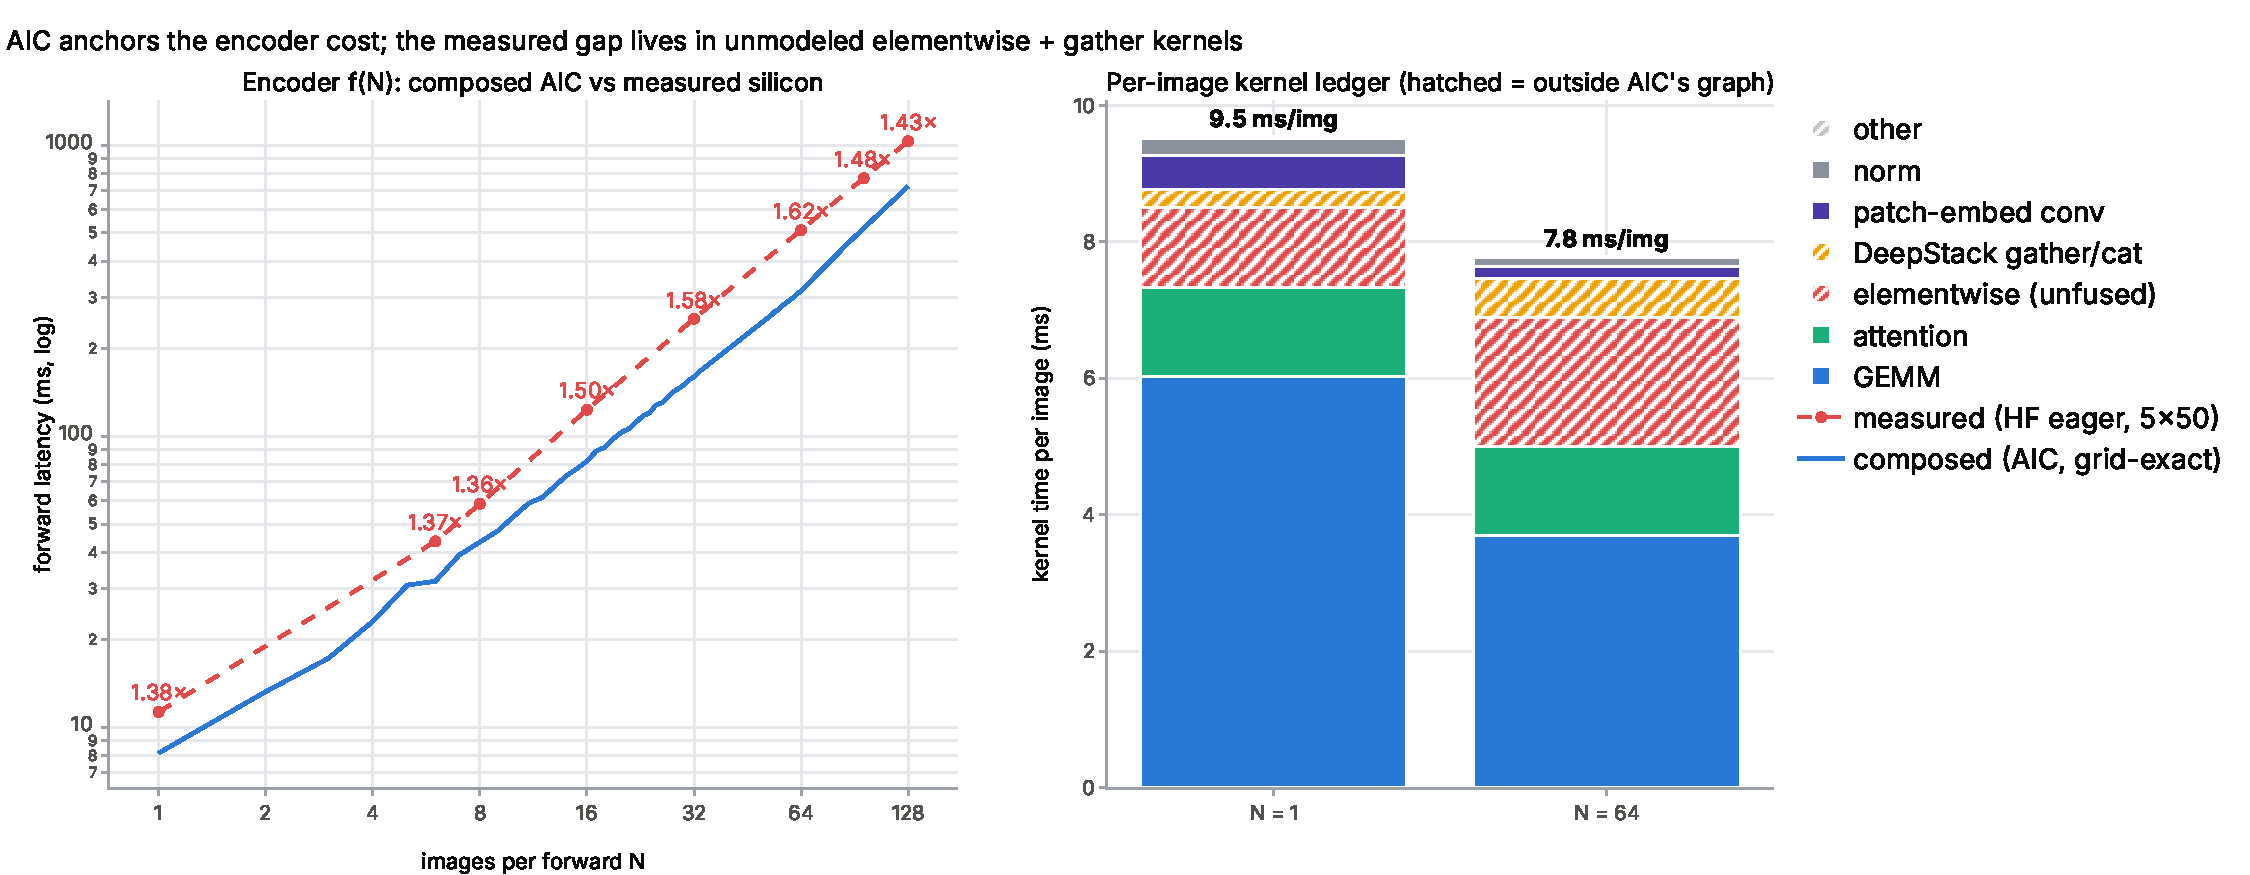
\includegraphics[width=\linewidth]{figuras/aic/aic_fn}
\caption[Composed $f(N)$ and the per-image kernel ledger]{Left: composed
$f(N)$ against end-to-end \emph{HuggingFace-eager} measurement (log--log,
ratio per point); the ratio rises with $N$, an execution-stack effect.
Right: the measured per-image kernel ledger at $N{=}1$ and $N{=}64$; the
hatched categories (unfused elementwise, DeepStack gather, patch-embedding
convolution) are HuggingFace-stack overhead outside AIC's operator graph,
and are what grows.}
\label{fig:aic-fn}
\end{figure}

\textbf{The HuggingFace-stack ratio grows with
$N$}, from ${\approx}1.37$ to $1.62$ at the 64-image dispatch cap: not
fixed overhead but \emph{per-image} work the operator graph omits. A
kernel-level profile at $N{=}64$ confirms it: the operators AIC models
behave exactly as composed (attention linear per image, per-image GEMM time
\emph{falling} as larger $m$ improves efficiency), while what grows is what
the HuggingFace forward carries \emph{around} those kernels: unfused
elementwise work, the DeepStack gather, and the patch-embedding convolution,
together \textbf{93\%} of the composition-vs-HuggingFace kernel-time
difference at $N{=}64$ (per-cell figures in Appendix~\ref{ap:artifacts}).

\textbf{That difference is a property of the execution stack, not of
AIC}. The operators AIC collects are vLLM's \emph{own} kernels (attention
through \texttt{vllm\_vit\_flash\_attn}, GEMMs through
\texttt{RowParallelLinear}), so the like-for-like anchor is vLLM's serving
forward. Measured directly, vLLM's complete Qwen3-VL vision tower matches
the composition to within \textbf{12.8\%} across the whole $N\le64$ serving
regime, whereas the HuggingFace forward is $1.4$--$1.6\times$ slower over
the same range. A dense $N{=}1$--$64$ sweep plus five off-cap probes
($N\in\{96,128,192,256,512\}$) confirms every batch up to the FIFO cap stays
within that bound; beyond the cap the composition under-prices vLLM, a
regime the pool never batches into. The check is forward compute on
synthetic inputs, not the full serving path; the four-engine sweep is in
Appendix~\ref{app:engine-sensitivity}. Batching benefit saturates by
$N{\approx}6$--$8$ on both measured engines (per-image cost bottoms
${\approx}1.57\times$ below single-image, then drifts back up), bounding the
useful dispatch batch. Because measured vLLM cost matches the composition
across the serving regime, the AIC-priced worker sizing used in
Chapter~\ref{cap:closedloop} carries no separate silicon penalty.

\subsection{Physical validation at batch one}
\label{sec:aic-validation}

The validation target is the vision encoder of
\texttt{Qwen/Qwen3-VL-8B-Instruct}: a 27-block ViT (hidden size 1152, 16
heads of dimension 72, GELU MLP of width 4304), a PatchMerger projector into
the language model's \num{4096}-dimensional embedding space, and three
DeepStack mergers. The family shares this tower across its 8B, 32B, and 235B
variants~\cite{Qwen3VL2025}, so the encoder result transfers across it: the
235B shares the 4096-dimensional projector target unchanged, and the 32B's
5120-dimensional projector scales only its final GEMM and handoff bytes,
leaving the tower-dominated cost model intact. The tower was extracted into
a standalone module field-by-field identical to the configuration AIC's
graph is built from, so prediction and measurement describe the same
network; measurement uses CUDA events around the full forward pass (patch
input resident on GPU), bf16, 5 replications of 50 timed iterations.

\begin{table}[htbp]
\centering
\caption[Encoder forward: measurement versus AIC prediction]{Vision-encoder
forward latency: measurement vs.\ AIC prediction (RTX~5090, bf16, batch 1,
SM clock locked, delivered 2385--2392\,\si{\mega\hertz}). Predictions from
the \emph{raw slice} (Section~\ref{sec:aic-collection}); 95\% $t$-intervals
across five replications.}
\label{tab:aic-validation}
\begin{tabular}{lrrrr}
\toprule
Image size & Patches & Measured (ms) & Predicted (ms) & Ratio \\
\midrule
$448^2$  & 784   & $11.360 \pm 0.006$  & 7.822  & 1.45 \\
$896^2$  & 3136  & $36.421 \pm 0.010$  & 31.973 & 1.14 \\
$1344^2$ & 7056  & $103.824 \pm 0.022$ & 89.347 & 1.16 \\
\bottomrule
\end{tabular}
\end{table}

\textbf{The analytical model matched the empirical test}: a kernel-level
profile accounts for the gap term by term, except a ${\approx}0.7$\,ms
remainder. At $448^2$, wall time decomposes into CUDA kernel time plus
inter-kernel dispatch gaps (15.3\%), a HuggingFace-eager property outside
AIC's scope. Within kernel time the attention kernels agree with prediction
to \textbf{within ${\approx}3\%$} on the collected operator, and the GEMM
total runs ${\approx}6\%$ high (HuggingFace selects different cutlass
variants than vLLM's path). Two modules sit outside AIC's graph altogether:
the patch-embedding convolution (an inefficient shape, far costlier than
its FLOPs suggest) and the DeepStack gather. Removed, they leave
AIC-comparable work within ${\approx}12\%$ of prediction. The DeepStack
merger MLPs themselves \emph{are} modeled: forcing the projector instance
count from four to one rescales predicted projector cost by exactly the
$4.00\times$ instance ratio. Consistent with this, the gap shrinks from $1.45\times$ at $448^2$ to
$1.14$--$1.16\times$ at larger images as fixed per-layer dispatch overhead
amortizes over longer kernels. Per-term kernel figures are in the provenance
manifest (Appendix~\ref{ap:artifacts}).

\subsection{Physical replay of controller-arm dispatch}
\label{sec:aic-physical-replay}

The batch-one and $f(N)$ checks above validate the encoder \emph{cost
model}; a final check validates the \emph{controller-arm delay verdicts}
that model produces. One GPU cannot host a time-shared fleet without
distorting physics, so the test is a trace-driven physical replay: each
arm's exact batch dispatch sequence for the fastest-onset burst window
(ledger key \texttt{burst3}) is regenerated from the frozen simulation
artifacts, gated against the banked statistics (batch, forward, image,
busy-time, and delay-percentile counts must match exactly), and executed
batch-for-batch on the physical encoder (the extracted tower of
Section~\ref{sec:aic-validation}, RTX~5090, bf16, clock-gated at
${\geq}2377$\,\si{\mega\hertz}). A frozen-composition retiming then holds
batch membership and worker schedule fixed while recomputing start and
finish times from the \emph{measured} per-batch service, yielding a
physically-timed per-request encoder delay. Composition is deliberately not
allowed to re-form, so this is a retiming, not a closed-loop
re-simulation; the measured per-$N$ table supplies a second
frozen-dispatch service representation for sensitivity, and does not test
composition re-formation.

The replicate estimand is the per-repetition retimed delay p99; five
predeclared repetitions per arm, reported as mean~$\pm$ sample standard
deviation. Under the HuggingFace-eager execution stack the forecast arm
retimes to $782.455 \pm 0.270$\,ms --- inside the \SI{1}{\second} bound
--- while the floorless reactive arm retimes to $22{,}565.317 \pm
0.935$\,ms, a ${\approx}29\times$ separation that dwarfs within-arm
variation: \textbf{the simulated forecast-versus-reactive delay verdict for
this window survives physical retiming} on the named engine and hardware.
The static arm breaches under HuggingFace-eager ($1{,}397.413 \pm
1.140$\,ms), but the like-for-like anchor for feasibility is the vLLM
serving stack AIC's kernels target: exact queue retimes through the
measured vLLM per-batch service keep static-$C{=}8$ feasible
(\num{745.758}\,ms direct, \num{747.169}\,ms per-$N$ simulator-scaled,
against \num{717.755}\,ms stored simulation p99; the canonical phase-E
sweep governs these values, with the tier-5 replication sweep banked as a
side-by-side sensitivity). The HuggingFace-eager
numbers are therefore the higher-latency measured sensitivity case on the
tested shapes --- an execution-stack effect, consistent with the
$1.4$--$1.6\times$ stack ratio above --- not a conservative bound, which
would require an ordering argument over engines these measurements do not
supply.

The same protocol was applied to the opposite regime: a calm 24-hour slice
(ledger key \texttt{steady24h}; five repetitions per arm), which
dispatches mostly single-image batches (p50 $N{=}1$) --- the small-$N$ end
of $f(N)$, the corner the burst window does not exercise. In the banked
simulation all three arms sit inside the bound (static \num{418.205},
forecast \num{681.117}, reactive \num{684.999}\,ms). Across the three
service representations, static remains the lowest-p99 arm and the two
controller arms remain near-tied at p99 (a 3.9\,ms simulator gap that
becomes an exact order-statistic tie under the measured vLLM service,
and a $0.037$\,ms difference of five-repetition means under
HuggingFace-eager whose sign flips between repetitions). Under the
canonical vLLM representations, every arm passes the calm day
(forecast/reactive \num{738.751} direct and \num{742.587} per-$N$
scaled; static \num{434.516}/\num{435.497}\,ms). Under
HuggingFace-eager the two controller arms cross the bound
($1{,}120.967 \pm 0.456$ and $1{,}121.004 \pm 0.143$\,ms) while
static does not ($610.596 \pm 0.175$\,ms) --- the absolutes are
engine-band-conditional, as on the burst window. No equivalence margin
was predeclared, so the forecast arm is reported as having no resolved
p99 separation from reactive in this experiment, not as equivalent to
it; against the overprovisioned static arm both controller arms trade
delay headroom for the worker-hour savings quantified in
Chapter~\ref{cap:closedloop}.

Scope is equally narrow in the other directions: the replay anchors
\emph{encoder delays only} (resource-time economics remain simulated by
construction), a single physical unit retimes a simulated multi-worker
schedule, and windows without settled physical cells carry no physical
claim. Every included repetition passes exact membership recovery
(1{,}241/1{,}241 requests on the burst window; 37{,}672/37{,}672 on the
calm day) and reconstruction of the banked simulation percentiles within
the declared numerical tolerances, and a negative-gate suite asserts that corrupted
membership, reordered dispatch, or changed engine, model, or clock
fingerprints fail loudly rather than silently retime
(Appendix~\ref{ap:artifacts} pins every raw artifact at the settled
evidence commit).

\section{Two-pool composition and fidelity}
\label{sec:aic-twopool}

Composing the calibrated encoder model with \texttt{dynamo.replay} yields
the running system the remaining experiments use. Three fidelity properties
follow: what calibrated language timing changes, what the encoder cost model
admits exactly, and where each pool saturates.

\subsection{Language-pool timing: the polynomial hides the tails}
\label{sec:sim-timing}

Table~\ref{tab:sim-poly-aic} compares the two timing models on the same
2{,}000-request steady window (raw arrivals, identical topology). The
calibrated model is moderately slower on averages and markedly heavier in
the tails: TTFT p99 grows $1.24\times$, and maximum TTFT and inter-token
latency roughly double ($1.8\times$, $1.9\times$). Burst behavior, what
autoscaling experiments measure, is visible only under calibrated timing, so
all headline runs use AIC timing and the polynomial is retained for cheap
coverage sweeps. These AIC numbers come from the source-built runtime, whose
predictions run in-core (Rust) in microseconds; an earlier wheel-based
runtime ran them as per-request Python callbacks whose wall-time leaked into
the simulated clock and inflated the extreme tail, an instrumentation
artifact to guard against whenever a timing hook is slower than the events
it prices.

\begin{table}[htbp]
\centering
\caption[Language pool: polynomial versus calibrated timing]{Language pool
under identical load and topology, polynomial vs.\ calibrated (AIC
\texttt{h100\_sxm}, vLLM 0.22.0) timing; 2{,}000-request steady window, 2
workers, offline KV router. AIC column from the source-built runtime;
provenance in Appendix~\ref{ap:artifacts}.}
\label{tab:sim-poly-aic}
\small
\begin{tabular}{lrr}
\toprule
Metric & Polynomial & AIC h100 \\
\midrule
TTFT avg / p99 / max (ms) & 67.3 / 248 / 2{,}540 & 68.2 / 307 / 4{,}518 \\
Request latency avg / p99 (ms) & 1{,}413 / 6{,}879 & 1{,}590 / 8{,}163 \\
Inter-token latency avg / max (ms) & 6.79 / 181 & 7.67 / 348 \\
Output tok/s per user (avg) & 160.6 & 142.0 \\
\bottomrule
\end{tabular}
\end{table}

\paragraph{Family transfer.} Language-pool numbers are for Qwen3-VL-8B at
TP1. Two run vintages price the flagship, Qwen3-VL-235B-A22B at TP8, on the
same shipped H100 data, window, and topology. The committed wheel-era spot
check (scales $s\in\{1,4,16\}$ only) measures ${\sim}1.9\times$ the 8B's
mean decode latency at the trace's own rate (1.3--3.8$\times$ across its
three scales), with ITL p99 \SI{87.7}{\milli\second} at that rate; the later
source-built 1.3.0 sweep reproduces that operating point
(\SI{86.2}{\milli\second}) and is the series that pins the knee, failing at
$s{=}2$ (\SI{210.6}{\milli\second}). The decode bound thus moves and the
flagship's knee drops to $s{=}1$ against the 8B's $s{=}2$: decoder scale
halves the language pool's operating envelope (both vintages' artifacts in
Appendix~\ref{ap:artifacts}). The vision side needs no such caveat: ViT and
4096-dimensional projector output are identical between the 8B and the 235B,
so the encoder cost model, batching law, burst-saturation result, and
handoff bound transfer unchanged.

\subsection{Encoder-pool realism: an exact batching law and a handoff bound}
\label{sec:sim-encoder}

\paragraph{Batching.} Probed directly, AIC's encoder graph prices a forward
\emph{exactly} by its total images: every factoring of $N$ images into
(batch, images-per-request), $(1,64)$ or $(64,1)$, returns the same
latency to the microsecond, because attention is evaluated at the product
batch$\times$images and every other operator at the total token count. Each
dispatched batch is costed at its image total, and batching pays: $f(1) =
\SI{8.16}{\milli\second}$ per image alone versus
$f(64) = \SI{316.4}{\milli\second}$, i.e.\ \SI{4.94}{\milli\second} per
image amortized, a $1.65\times$ throughput gain. (End to end the realized
gain is smaller and saturates by $N{\approx}6$--$8$, which is conservative
for the saturation results below.) Dispatch is greedy FIFO: a freed worker takes
whole queued requests, in order, up to a 64-image cap (the collected batch
range, so no extrapolation); a request exceeding the cap alone, the trace
reaching $97^2 = \num{9409}$ images, is chunked into $\leq 64$-image
forwards entering the FIFO as independent units, so several free workers
drain one oversized request concurrently. Chunk-parallel dispatch is a
\emph{simulator policy assumption}: consistent with encoder-disaggregated
runtimes that route image groups independently across instances, physically
grounded (images are independent in the encoder), but not a property of the
trace. It makes encoder tail latency \emph{capacity-controllable}: under the
sequential alternative (chunks chained on one worker, retained behind a
converter flag) the largest requests carry an intrinsic multi-second service
time that no worker count removes, with delay p99 plateauing at
\SI{2.9}{\second} from 4 through 32 workers, making every frames-heavy
window statically infeasible by construction. The largest request costs
${\approx}\SI{46.5}{\second}$ of kernel time regardless. Under low load the
policy changes nothing; it matters inside bursts.

\paragraph{Handoff.} The encoder's output crosses pools, and the runs charge
the \emph{main} projector stream (post-merge vision embeddings, $196 \times
4096$ bf16 values, ${\approx}\SI{1.6}{\mega\byte}$ per image), bounded
analytically as $\text{RTT} + \text{bytes}/\text{bandwidth}$ on a
parameterized link (default \SI{25}{Gbps}): \SI{0.71}{\milli\second} at the
steady window's median request, \SI{62}{\milli\second} at its 121-image
maximum. Two caveats delimit the bound. First, a disaggregated Qwen3-VL
deployment must also ship the three DeepStack projections the language model
consumes in its early layers, quadrupling the payload to
${\approx}\SI{6.4}{\mega\byte}$ per image
(${\approx}\SI{250}{\milli\second}$ at that maximum); still second-order
against the multi-second queueing tails measured here, but a known
undercount for this family, whose $4\times$-payload sensitivity
Chapter~\ref{cap:closedloop}'s limitations quantify on the week-scale
aggregate. Second, the bound is \emph{bandwidth-only}: contention,
serialization, NIC/PCIe placement, and cross-node topology are unmodeled,
so it is a lower bound on transfer latency, not a tail estimate; it is
charged to request latency but not to the worker (asynchronous DMA/NIC), and
a measured NIXL curve can later replace it.

\subsection{Saturation knees: the decoupling, now in simulation}
\label{sec:sim-knees}

The platform can now answer the load question: \emph{at what offered load
does each pool violate its latency target?} Arrival timestamps are
compressed by a speedup factor $s$, natively in \texttt{dynamo.replay} for
the language pool (on the isolation trace, so the knee is attributable to
that pool alone) and in the converter for the vision pool. Two windows are swept at the
locked 2-encoder $\times$ 2-LLM topology: the steady 2{,}000-request head
(\SI{2.77}{req/s}, \SI{8.0}{img/s}) and the window enveloping the week's
largest burst episode (Section~\ref{sec:eda-vision}, padded $\pm$10 minutes:
64{,}804 requests over \SI{8.3}{\hour}, mean \SI{2.17}{req/s} but
\SI{116}{img/s}, peaking at \SI{370}{img/s}).

\begin{table}[htbp]
\centering
\caption[Saturation knees per pool and window]{Saturation knees under the
evaluation SLA: largest swept speedup $s$ meeting every bound, and that
knee's offered load. ``ITL-bound'' marks knees whose successor point still
meets the TTFT budget but crosses the inter-token bound. The vision pool's
steady-window knee is censored (never crossed within $s \leq 32$). Last
column: TTFT p99 for language rows, encoder-delay p99 for vision rows.
\emph{Provenance caveat:} the sweep set mixes source-built and wheel-based
runtimes (per-point attribution in Appendix~\ref{ap:artifacts}); the
tabulated knee is insensitive to this --- $s{=}2$ meets every bound and the
$s{=}3$ inter-token p99 breaches \SI{100}{\milli\second} outright.}
\label{tab:sim-knees}
\footnotesize
\setlength{\tabcolsep}{2pt}
\begin{tabular}{llrrr}
\toprule
Pool / timing & Window & Knee & Offered & TTFT / enc.\ delay p99 (ms) \\
\midrule
LLM / poly & steady & $s{=}3$ (ITL-bound) & 8.3 req/s & $248 \to 374$ \\
LLM / AIC  & steady & $s{=}2$ (ITL-bound) & 5.5 req/s & $307 \to 418$ \\
LLM / poly & burst & $s{=}1$ & 2.2 req/s & $910$ at $s{=}1$ \\
LLM / AIC  & burst & \textbf{none: over at $s{=}1$} & 2.2 req/s & $1{,}868$ at $s{=}1$ \\
Vision / AIC & steady & $\geq s{=}32$ (cens.) & $\geq$ 256 img/s & $199 \to 787$ \\
Vision / AIC & burst & \textbf{none: over at $s{=}1$} & 116 img/s & $5{,}013$ at $s{=}1$ \\
\bottomrule
\end{tabular}
\end{table}

\begin{figure}[htbp]
\centering
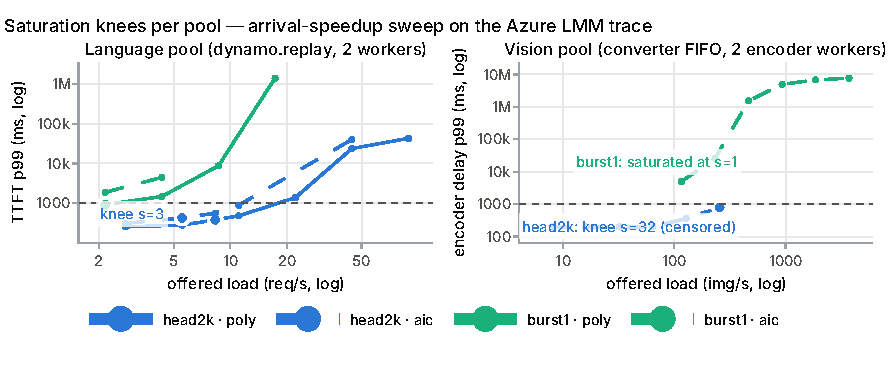
\includegraphics[width=\linewidth]{figuras/sim/sim_knees}
\caption[TTFT and encoder-delay p99 versus offered load]{TTFT and
encoder-delay p99 versus offered load per pool (log--log), swept by arrival
speedup at the fixed 2$\times$2-worker topology. Knee markers apply the full
evaluation SLA, so the steady-window language knees sit \emph{below} the
TTFT line: the inter-token bound crosses first. On the steady head (blue,
labeled \texttt{head2k} --- distinct from the 24-hour steady window) the
vision pool stays under its bound through $s{=}32$, and at the calibrated
language knee the encoder idles at 4.5\% utilization. On the burst window
(green) both calibrated curves start \emph{above} their bounds at the
window's own rate: language at 1.9$\times$ its TTFT bound, vision at
5$\times$ its delay bound.}
\label{fig:sim-knees}
\end{figure}

On the steady head the separation is an order of magnitude: the vision pool
is uncrossed at $32\times$ the trace rate while the language knee sits at
$s{=}3$ (polynomial) or $s{=}2$ (calibrated), the sweep being
octave-spaced above $s{=}4$: a factor ${>}10$ under calibrated timing, so
sizing both pools off one signal would overprovision the encoder fleet by
that factor in calm traffic. The dual-bound SLA adds a second structural
fact: that language pool is \emph{decode-bound}, not TTFT-bound. At the
knee's successor point the TTFT budget still has $1.8$--$2.1\times$ slack
while ITL p99 has crossed, so its capacity under an interactive SLA is
set by sustained token throughput per user, the axis the 235B spot-check
stresses further.

Inside the burst window, calibrated timing overturns the polynomial's
language verdict: the polynomial has the pool skirting its bound at the
window's own rate (\SI{910}{\milli\second}, 9\% under), while the same run
under AIC timing reads \SI{1868}{\milli\second}: the frames-class
requests' ${\approx}36$k-token prefills alone exceed the TTFT budget at TP1,
a \emph{prefill floor} persisting at any worker count (the baseline
chapter's grid finds TTFT p99 pinned near \SI{1.3}{\second} from 4 through
16 TP1 workers here). At the naive topology the burst thus breaks \emph{both}
pools, structurally differently. The language pool's is a per-request
compute floor, visible in any TTFT dashboard and removed by one static
parallelism decision: TP2 at the same worker count (four GPUs) passes the
window at \SI{748}{\milli\second} TTFT p99 and \SI{6.6}{\milli\second} ITL
p99. The vision pool's failure has no such fix: p99 encoder delay of
\SI{5.0}{\second} ($5\times$ the bound) from episodic queueing at 29\% mean
utilization, invisible to rate- and mean-utilization monitors (the
minute-mean stays low even as the 1-minute peak busy fraction reaches 0.90),
yielding only to capacity: six encoder workers, $3\times$ this topology,
at the trace's own rate.

Figure~\ref{fig:sim-burst-queue} exposes the mechanism. The window's
7{,}716 requests above the 64-image dispatch cap, the chunked population,
7{,}643 of them in the canonical frames class ($k{>}10$ grids), decompose
into chunk units of at most 64 images that, with smaller requests batched
behind them, drive 83{,}376 forwards; arrivals clump, the worst second
landing 2{,}726 images at once. Behind a strict FIFO a frames flood
monopolizes \emph{every} worker: the backlog exceeds 1{,}000 queued images
for 805 seconds across the eight-hour window, peaking at 4{,}701, each
excursion a multi-second p99 event, yet the pool drains fully between them.
Request rate, mean utilization, and conventional five-minute aggregate
summaries read healthy while the tail SLA is violated episodically all day
--- the invisibility is clean only near five-minute cadence, since on a
1-minute clock the image-driven busy fraction reaches 0.90 here, with 0.6\%
of one-minute windows above an 0.8 target. Catching that
requires watching, or forecasting, the image signal itself, at the
horizons Chapter~\ref{cap:predictors} shows to be forecastable.

\begin{figure}[htbp]
\centering
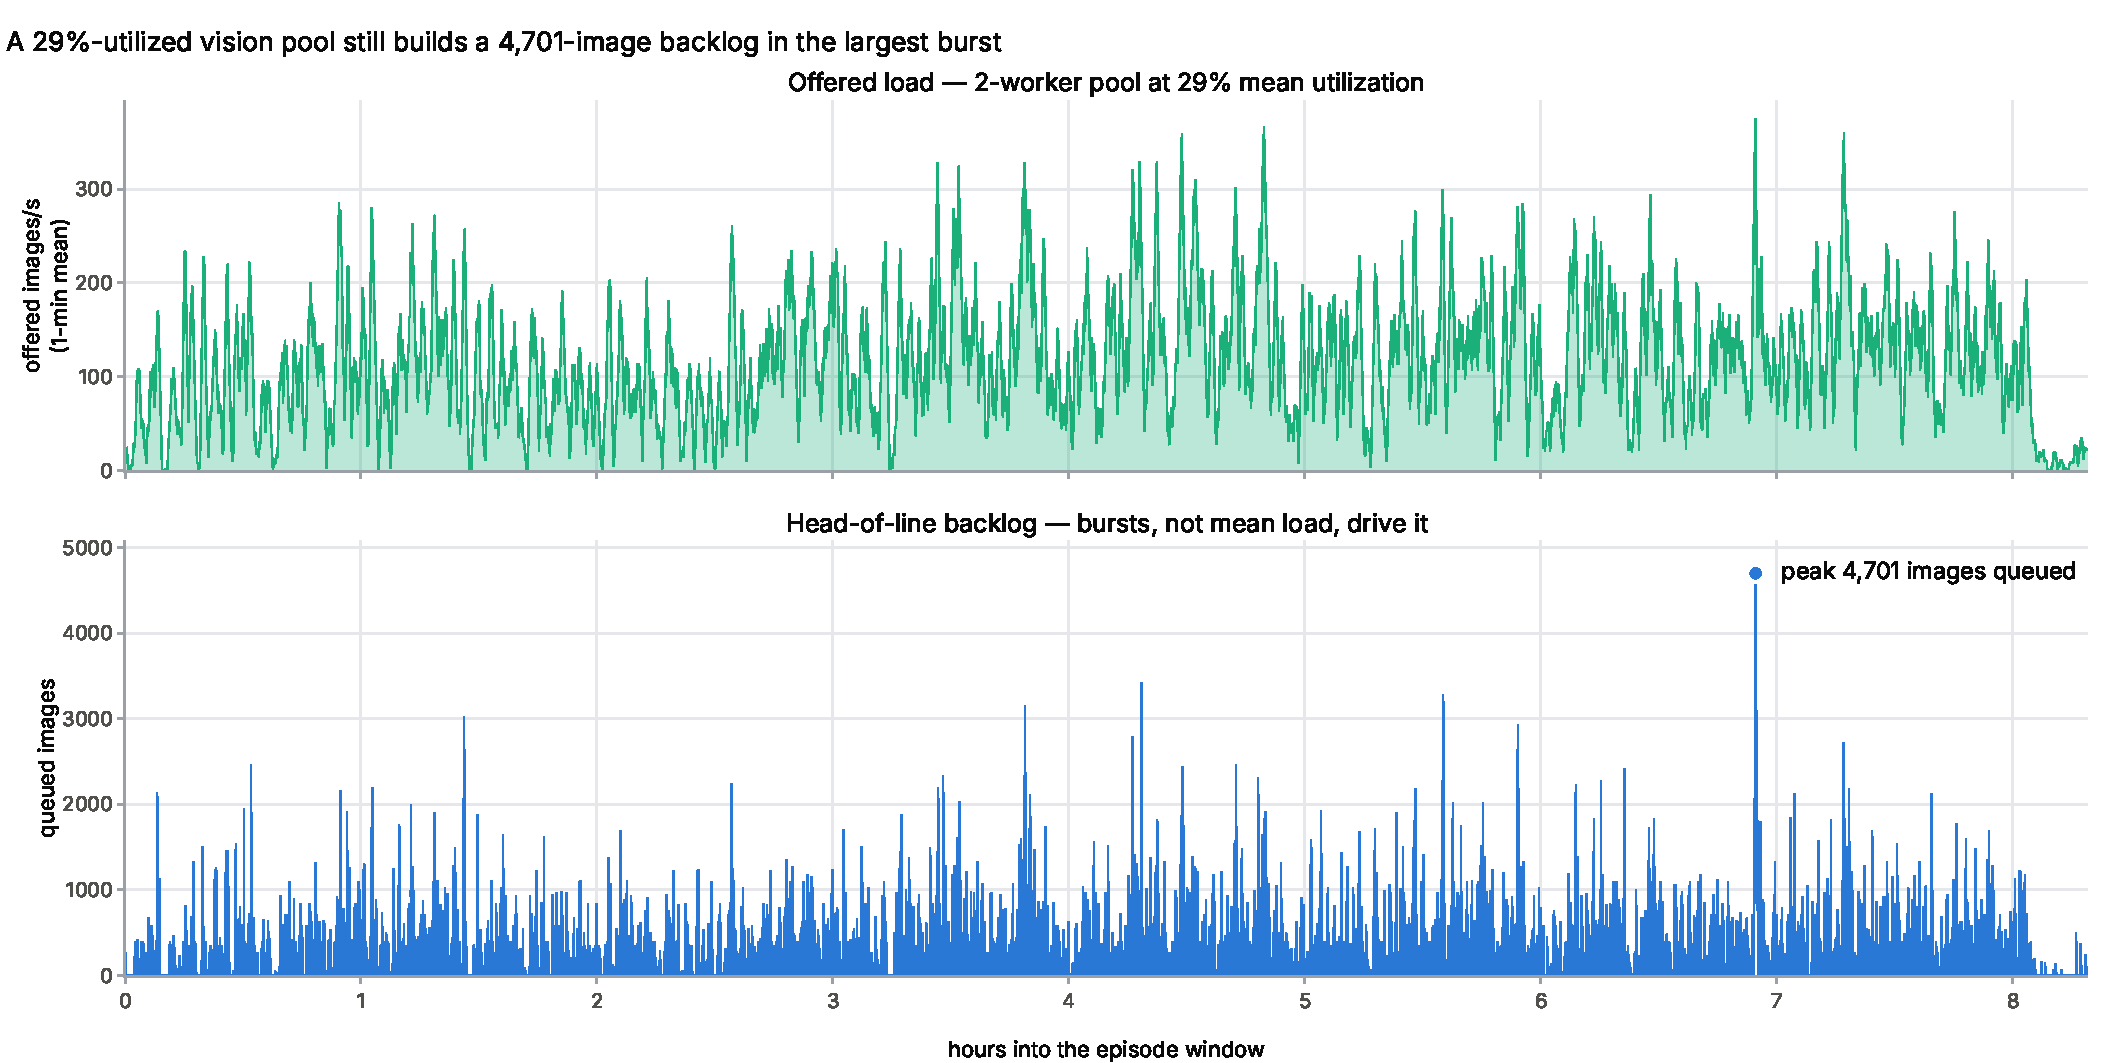
\includegraphics[width=\linewidth]{figuras/sim/sim_burst_queue}
\caption[Offered image load and encoder queue depth inside the burst
window]{Inside the burst window at the trace's own rate: offered image load
(top, 1-minute mean of the per-second series) and the encoder pool's
queued-image depth (bottom, per second). The queue repeatedly spikes and
fully drains between spikes --- the episodic FIFO head-of-line blocking
behind frames-class floods analyzed in the text.}
\label{fig:sim-burst-queue}
\end{figure}

\section[Live-stack anchor]{Live-stack anchor: the same loop on the real
control plane}
\label{sec:val-results}

Every closed-loop result runs through Dynamo's \emph{offline} replay: real
planner code, virtual clock, in-process actuation. The last fidelity
question the simulator cannot answer about itself is whether that loop
behaves the same on the live stack: HTTP frontend with in-process KV
router, independent mocker workers discovered over etcd, Prometheus metrics,
the SLA planner as its own service, and scaling actuated through the
planner's VirtualConnector protocol by a worker-manager written for this
thesis. This is fidelity evidence for the platform, not a result about the
contribution.

\subsection{Setup}
\label{sec:val-setup}

The anchor window is the one-minute-onset window burst3 (the hardest
case in the fleet matrix; the window set is declared in
Section~\ref{sec:cl-contract}), replayed in real time (\SI{27}{\minute}, 3{,}093
scheduled requests) by a fixed-schedule load client (aiperf) that
synthesizes each request at its trace timestamp with its exact token counts
and prefix-sharing structure, measuring TTFT/ITL client-side. Both policies
run the production planner service: the \emph{forecast} policy is the
thesis's winning configuration (archived Chronos p90 path at 15-second bins
through the \texttt{forecast\_file} predictor, tail-aware conversion,
60-second replica lead); the \emph{reactive} policy is the variant-B
baseline (ARIMA predictor, 200/20\,ms window-mean targets). Engine timing is
identical to the offline runs by construction: live mocker workers load the
same AIC latency model, engine arguments, and KV-block capacity, one TP2
replica per OS process so replicas die independently. The cold-start lead is
modeled by delayed spawn (59\,s + a measured 1.0\,s spawn-to-registered
latency), mocker-native \texttt{startup\_time} being unusable because its
live semantics \emph{invert} the offline ones
(Section~\ref{sec:val-findings}). Each live run is compared against an
offline twin: identical trace, planner configuration, capacity mapping,
lead, and budget, re-run through the replay platform above.

\subsection{Verdicts, tails, and decisions agree}

\begin{table}[htbp]
\centering
\caption[Live stack versus offline twin on burst3]{Live stack versus offline
twin on burst3 (evaluation SLA: TTFT p99 $<$ \SI{1}{\second}, ITL p99 $<$
\SI{100}{\milli\second}; budget-matched at 4 TP2 replicas). ITL p99 is the
per-request inter-token latency
$(\text{RequestLatency}-\text{TTFT})/(\text{OSL}-1)$ computed like-for-like
in both columns, matching aiperf's live metric and Dynamo's SLA definition
(ITL${=}$TPOT). Live tails are computed over successful responses ---
3{,}092 of the 3{,}093 scheduled for the forecast run and 3{,}089 for the
reactive run (1 empty-response error and 4 HTTP-500s, respectively) --- so
the verdicts grade latency on completed requests, not availability.}
\label{tab:val-anchor}
\small
\begin{tabular}{@{}llrrr@{}}
\toprule
Policy & Metric & Live & Offline twin & $\Delta$ \\
\midrule
Forecast p90 & TTFT p99 (ms) & 695 & 651 & $+6.8\%$ \\
 & ITL p99 (ms) & 11.5 & 9.7 & $+1.8$\,ms \\
 & replica-seconds & 6{,}063 & 6{,}400 & $-5.3\%$ \\
 & verdict & \textbf{PASS} & \textbf{PASS} & agree \\
\midrule
Reactive & TTFT p99 (ms) & 3{,}531 & 3{,}495 & $+1.1\%$ \\
 & ITL p99 (ms) & 150.7 & 152.7 & $-1.3\%$ \\
 & replica-seconds & 1{,}799 & 1{,}948 & $-7.6\%$ \\
 & verdict & \textbf{FAIL} & \textbf{FAIL} & agree \\
\bottomrule
\end{tabular}
\end{table}

The anchor holds in both verdict directions (Table~\ref{tab:val-anchor}):
the forecast policy passes the tail SLA live exactly as simulated, the
reactive policy fails likewise with its p99 within 1.1\% of the simulation,
and provisioned replica-time agrees within 8\%. The agreement extends below
the aggregates. The \emph{demand} path is byte-identical: for the first
twelve planner ticks, live and offline planners log the same predicted demand
to the second decimal (first tick \texttt{29.86 rps} in both, both computing
\texttt{6 replicas}), predictor, registry, construction order, and demand
conversion being the same code with only the clock differing. The
\emph{capacity} belief already differs at the first tick (live \texttt{5.71}
versus offline \texttt{5.30 engine\_rps}, both still yielding 6 replicas)
and drifts within its expected band throughout, its regression being tuned
from sampled forward passes that arrive in a different order live; but the
\emph{applied} capacity, after the budget cap, tracks the same trajectory.
Client-observed TTFT tails land within 1.1--6.8\% of the simulated ones (a
single live run per policy, so this is a point difference between two
systems, not a repeated-run noise band). The policy split on this window
reproduces on the real stack in the two policies carried live: the p90 forecast passes
where the reactive baseline fails (the failing p50 leg is established
offline only, Chapter~\ref{cap:closedloop}).

\subsection{What the live stack revealed}
\label{sec:val-findings}

The anchor's second product is the divergences it surfaced. None is
policy-level; all are worth knowing before a deployment:

\begin{description}
\item[Live \texttt{startup\_time} inverts the offline semantics.] Offline it
keeps a scal\-ing-up mocker invisible to the router until ready; live it
registers the worker \emph{immediately} and stalls its requests, opening a
routable-but-dead window that a load-aware router, seeing an idle-looking
worker, preferentially fills. Hence the delayed-spawn modeling above.
\item[The live capacity model starves at calm load.] The live planner
samples worker metrics in tracking mode (the \emph{latest} forward pass per worker,
once per load tick) while the offline replay feeds \emph{every} pass. Mixed
prefill+decode passes, the only samples informing aggregated capacity, are
rare at calm load (only ${\approx}1\%$ of calm-load samples), too few
to make the model ready, so it would warm only once the workload was already
busy, too late for scale-ahead decisions. The fix (contributed to the Dynamo
tree as an opt-in \texttt{fpm\_observation\_mode}) drains every published
pass into the same regression feed the replay uses; with it the live planner
is ready at its first tick and computes the offline twin's first decision.
\item[Tick cadence stretches under stall.] The 60-second ticks held cadence
except one ${\approx}120$-second stall, after which the forecast feed
realigned to wall time; the offline virtual clock can never stall. Decision
\emph{count} is therefore not exactly reproducible live; decision
\emph{values} at matching times are.
\item[Budget units differ between paths.] The offline replay caps replicas
at \texttt{max\_\allowbreak gpu\_\allowbreak budget}; the live planner divides the same field by
GPUs-per-replica, and the anchor equalizes the caps. The cap \emph{does}
bind here: the tail-aware forecast requests up to 11 language replicas
against the equalized four-replica (8-GPU) cap, so it reshapes the
provisioned count, not the pass/fail verdict; the unit mismatch remains a
reportable upstream defect.
\end{description}

\subsection{Scope of the anchor}
\label{sec:val-scope}

The anchor covers one window (the hardest), two policies (the contribution
and the baseline it beats), the language pool (the pool with a production
control path; the encoder pool's controller exists only in simulation), and
mocked engine execution. It validates the \emph{control loop}, not GPU
silicon, which Section~\ref{sec:aic-validation} anchored physically on the
encoder side. Within that scope, closed-loop
behavior transfers to the real stack in both verdict directions: SLA
verdicts agree on both graded metrics, TTFT and provisioned replica-time
agree within single-digit percent, and the forecast policy's ITL differs by
\SI{1.8}{\milli\second} (18\%, on a \SI{9.7}{\milli\second} base, far under
the \SI{100}{\milli\second} bound). The divergences that do exist
(identified, explained, one fixed on a local branch to be proposed upstream)
are properties of the harnesses, not of the policies compared here.

\section{Fidelity caveats and limitations}
\label{sec:sim-limitations}

This section is the thesis's single canonical statement of platform
fidelity; later chapters reference it rather than restating it.

\emph{Timing fidelity is asymmetric between the pools.} The encoder model is
collected and physically validated on this thesis's own silicon
(Section~\ref{sec:aic-validation}); the language pool's calibrated timing is
trusted from AIC's shipped \texttt{h100\_sxm} database and Dynamo's engine,
and is not, and within this work cannot be, re-validated against
physical H100 measurement. The polynomial-versus-AIC comparison quantifies
the conclusions' \emph{sensitivity} to that timing model, which is not the
same as its accuracy: the steady-window knee moves by one sweep step and the
burst verdict changes outright. One pricing caveat follows from the
composition strata: the \texttt{h100\_sxm} context-attention grid stops at
\num{16384}-token inputs, so the ${\approx}3.1\%$ of trace requests beyond
it (up to ${\approx}149$k tokens, a share counted under the trace-token
convention) are priced by extrapolation, including the frames-class
prefills that decide the burst-window TTFT tail.

\emph{Per-request token accounting mixes conventions, with aligned biases.}
The simulation costs encoder work as a full $448^2$ forward per image and
ships $196 \times 4096$ post-merge values per image across the seam, but
sets the language pool's prefill length to the trace's
\texttt{ContextTokens} verbatim, which embeds the \emph{traced} model's
vision tokenization (${\approx}66$ tokens per image,
Chapter~\ref{cap:trace-eda}), roughly $3\times$ below a Qwen3-VL-consistent
196-per-image prefill. Frames-class language work is thus undercounted
(making the language pool look better in bursts) while the uniform $448^2$
assumption overstates frames-class encoder work (making the vision pool look
worse); both biases lean toward the burst asymmetry above. The TP1 prefill
floor is robust to them (it worsens at $3\times$ the tokens); the TP2 margin
is not. The burst-window language verdict is therefore
convention-dependent while the vision verdict is not, and a
both-conventions sensitivity run remains future work.

\emph{Image size is assumed, not recorded.} All encoder timing derives from
a single RTX~5090 node (locked clocks), so cross-unit silicon variance is
unquantified, and because the trace records no image sizes the uniform
$448^2$ assumption can only be stress-tested, not validated. When the
encoder is repriced at other resolutions through the collected operator
database (per-cell numbers in Appendix~\ref{ap:artifacts}), the
burst-window verdict holds at $448^2$
and below on both modeled fabrics, with the no-queue service time crossing
the bound near 690--705\,px, so the assumed resolution sits just below it.
A structural finding follows: provisioned worker-time is
\emph{invariant} across image size, because the schedule is driven by image
\emph{count} and is blind to \emph{size}. A size increase arrives as pure
service-time inflation with no provisioning response, unlike the engine-cost
gap above, which p90 headroom absorbs with no added workers. Two scope
limits bind: the $672^2$ margin on the faster fabric is thin and reflects
the single-stream handoff assumption, and under the plain forecast schedule
at issued lead $L{=}\SI{30}{\second}$ (artifact \texttt{fc\_L30}) on the
sustained 24-hour window $672^2$ misses the bound
on \emph{both} fabrics (the forecast-aware variant and the deployable
static-$C{=}8$ reference still meet it on the faster fabric,
\SI{842}{\milli\second}), so that fabric margin is a burst-window result
and must never be quoted without its window ($896^2$ cells extrapolate
beyond the collected batch axis, and every size distribution is
\emph{assumed}).

\emph{Scope of the simulated system.} The SLA's specific bounds
(\SI{1}{\second}/\SI{100}{\milli\second}/\SI{1}{\second}) follow the
interactive-serving convention rather than this trace: a first-token budget
of about one second keeps an exchange conversational, following the classic
interactive-latency envelope~\cite{Dean2013TailAtScale} and the TTFT range
the disaggregated-serving literature grades
against~\cite{Zhong2024DistServe,Patel2024Splitwise}; a
\SI{100}{\milli\second} per-token gap sustains generation at or above
human reading speed, the standard TPOT/ITL
rationale~\cite{Zhong2024DistServe}; and the encoder bound reuses the same
one-second budget because, through the composed seam, encoder delay
postpones the first token one-for-one, so the pre-LLM stage is graded on the
interactivity scale it consumes. They remain a design choice: knee positions
shift with them (under a lax TTFT-only \SI{2}{\second} bound the language
knees sit one to two octaves higher), though the sweep curves are SLA-free
and re-derivable under any bounds, and Section~\ref{sec:cl-frontier} grades
the frontier arms with the threshold swept.
Language-pool results are reported for the 8B at TP1, with a TP2$\times$2
spot-check on the burst window and a 235B-TP8 spot-check
(Section~\ref{sec:sim-timing});
intermediate family members (32B) were not priced.
The dispatch cap is not the source of the burst verdict (verified across
caps 32/64/128); the handoff term remains the bandwidth-only,
DeepStack-undercounting bound of Section~\ref{sec:sim-encoder}. Request
ingress (image fetch/decode, preprocessing, tokenization, front-end
queueing) is not simulated; the boundary is accelerator-side service and
queueing. Encoder delays fold into language-pool arrivals through the trace
seam, which serializes the pools per request; this is conservative for
composed TTFT, since overlap could only lower it. Per-pool knees were measured with
the other pool absent, making them attributable; composed-system claims are
made only where composed runs exist. The steady head used in the sweeps is
vision-lean (2.9 images per request against the trace's ${\approx}14$),
which the 24-hour steady window partly mitigates, raising the rate to 5.3,
still well below the trace-wide 14.3. Finally, the live anchor's engine
execution is mocked: it validates control-plane behavior, not GPU
throughput, and one burst replayed through real encoder workers remains the
outstanding fidelity upgrade.

\bigskip
\noindent
With the platform calibrated, its evaluation contract fixed, and its
fidelity bounded, the three research questions can be asked of it in turn:
whether request rate is an adequate proxy for vision demand
(Chapter~\ref{cap:trace-eda}), whether encoder demand is forecastable at
replica-startup horizons (Chapter~\ref{cap:predictors}), and whether
forecast-informed capacity placement under startup delay improves the
window-level trade-off between tail SLA and resource-time
(Chapter~\ref{cap:closedloop}).
